% Uncomment for Draft mode:
%\documentclass[onecolumn,pre,floats,aps,amsmath,amssymb,superscriptaddress]{revtex4-1}

% Journal mode, two columns
%\documentclass[twocolumn,pre,floats,aps,amsmath,amssymb,superscriptaddress]{revtex4-1}

% Journal mode, one column: 
\documentclass[onecolumn,pre,floats,aps,amsmath,amssymb,superscriptaddress]{revtex4-1}

% Edit mode, one column:
%\addtolength{\evensidemargin}{3in}
%\addtolength{\textwidth}{-2in}

\usepackage{layouts}
\usepackage[utf8]{inputenc}
\usepackage{amsmath}
\usepackage{amsfonts}
\usepackage{amssymb}
\usepackage{graphicx}
\usepackage{svg}
\usepackage[margin=0.725in]{geometry}

\DeclareMathOperator{\relu}{ReLU}

\begin{document}
\title{Using context to make gas classifiers robust to sensor drift}

\author{Jamieson Warner}
\affiliation{Department of Neuroscience, The University of Texas at Austin, Austin, TX}
\author{Ashwin Devaraj}
\author{Risto Miikkulainen}
\affiliation{Department of Computer Science, The University of Texas at Austin, Austin, TX}

% Uncomment for journal mode
\begin{abstract}
\textbf{\abstractname.} The interaction of a gas particle with a metal-oxide based gas sensor changes the sensor irreversibly. The compounded changes, referred to as sensor drift, are unstable, but adaptive algorithms can sustain the accuracy of odor sensor systems. This paper shows how such a system can be defined without additional data acquisition by transferring knowledge from one time window to a subsequent one after drift has occurred. A context-based neural network model is used to form a latent representation of sensor state, thus making it possible to generalize across a sequence of states. When tested on samples from unseen subsequent time windows, the approach performed better than drift-naive and ensemble methods on a gas sensor array drift dataset. By reducing the effect that sensor drift has on classification accuracy, context-based models may be used to extend the effective lifetime of gas identification systems in practical settings.
\end{abstract}

\maketitle

\begin{figure}
	\centering
	\frame{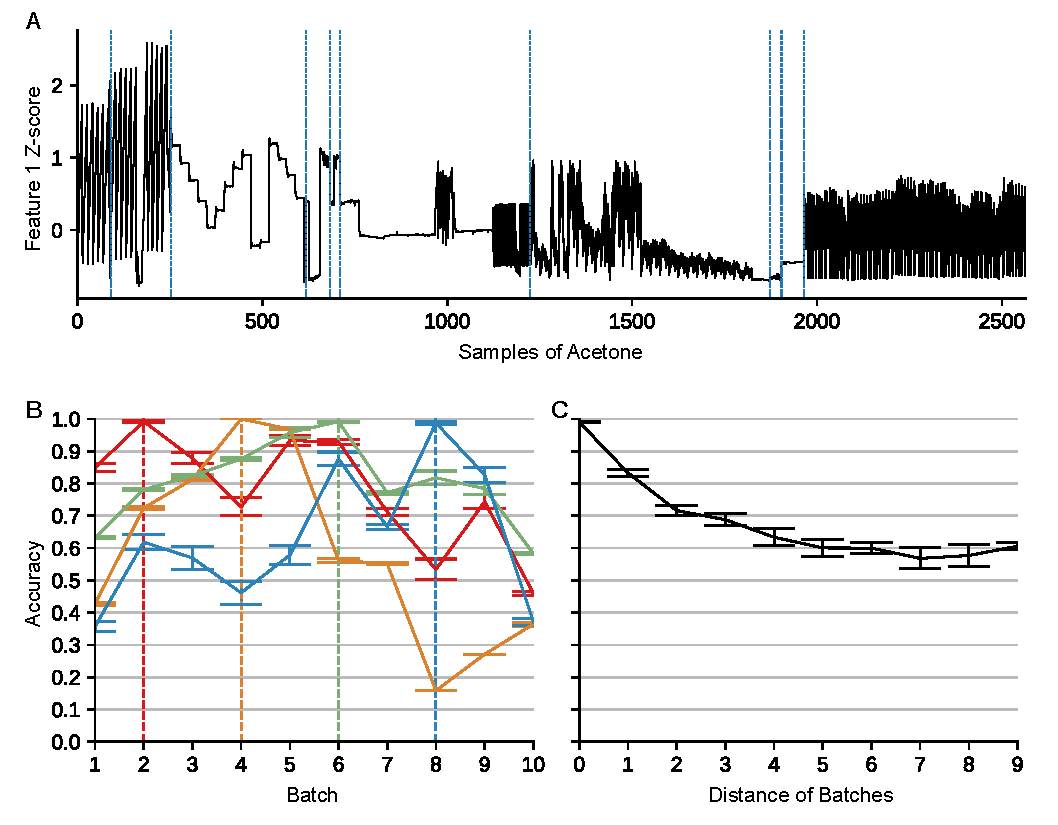
\includegraphics{fig_1.pdf}}
	\caption{\textbf{Recognizing odor despite sensor drift.} (\textbf{A.}) The first sensor feature dimension is plotted for all samples of the gas acetone. Vertical dashed lines mark the boundaries of the ten batches. There is variability within as well as between batches. (\textbf{B.}) For thirty trials, four feedforward networks are trained using a single batch of training data indicated by the vertical dashed lines and colors. The mean classification accuracies evaluated on each batch are shown along with 95\% confidence interval. The variability of response to a single odor poses a challenge to odor recognition. (\textbf{C.}) Mean accuracy along with 95\% confidence interval is shown as a function of the absolute distance between the training batch and the evaluation batch. The further away the testing batch is from the training batch, the lower the generalization accuracy becomes.}
\end{figure}
\section{Introduction}
Sensation of chemical gases in industry is mostly tasked to metal oxide-based sensors, chosen for their low cost and ease of use \cite{dickinson_current_1998,barsan_metal_2007}. An array of sensors with variable selectivities, coupled with a pattern recognition algorithm, readily recognizes a broad range of odors. The arrangement is called an artificial nose since it resembles the multiplicity of sensory neuron types in the nasal epithelium. While metal oxide-based sensors are economical and flexible, they are unstable over time.

Changes to the response properties of sensors, called sensor drift, hinder the sustained accuracy of odor identification and detection systems, drawing efforts to adapt to sensor change \cite{marco_signal_2012}. One technique to maintain classification performance after a sensor has been modified is to recalibrate the system with new odor samples. It is costly to collect and label such new samples because a skilled operator is needed, and the experimental conditions need to be controlled precisely \cite{marco_signal_2012}. Recalibrating a model with unlabeled examples, called unsupervised learning, is a possible alternative but difficult to establish in practice. Alternatively, a gas classifier may retain accuracy by being robust to sensor drift, which is the approach taken in this paper. The focus is extending the lifetime of sensor systems without recalibration, measured by generalization to unseen data recorded after sensor drift.

In natural settings, odor identification is a complex task. Natural odors consist of complex and variable mixtures of molecules present at variable concentrations \cite{thomas-danguin_perception_2014}. Sensor variance arises from environmental dynamics of temperature, humidity, and background chemicals, all contributing to concept drift \cite{vito_pattern_2016}, as well as sensor drift araising from modification of the sensing device. The hard problem of olfaction in nature calls for the learning of new odor assocations \cite{imam_rapid_2019}. In an attempt to capture much of this complexity, Vergara et al. \cite{vergara_chemical_2012} developed a publicly available benchmark dataset demonstrating sensor drift over a period of 36 months. This dataset offers a controlled testbed for sensor drift mitigation algorithms and thus defines the scope of this paper. 

This paper builds upon previous work with this dataset, i.e., Vergara et al. \cite{vergara_chemical_2012}, which used support vector machine (SVM) ensembles. First, their approach is extended to a modern version of feedforward artificial neural networks (NNs) \cite{pardo_remarks_2004}. Context-based learning is then introduced to utilize sequential structure across batches of data. The context model has two parts: (1) a recurrent context layer, which encodes classification-relevant properties of previously seen data, and (2) a feedforward layer, which integrates the context with the current odor stimulus to generate an odor class prediction. The results indicate improvement from two sources: the use of neural networks in place of SVMs, and the use of context, particularly in the cases when a substantial number of context sequences are available for training.

\section{Related Work}
Our contribution should be considered in the context of the substantial body of work training models in nonstationary environments (Section \ref{section:review-sensor-drift}). We also review circuit models of context-aware odor processing in biological systems, from which this work draws inspiration (Section \ref{section:review-biological-olfaction}).

\subsubsection{Sensor drift adaptation}
\label{section:review-sensor-drift}


\subsubsection{Use of odor context in the mammalian olfactory system}
\label{section:review-biological-olfaction}
The mammalian olfactory system, which tackles the challenges of natural olfaction, often inspires odor processing algorithms \cite{marco_recent_2009}. One example is the KIII model, a dynamic network resembling the olfactory bulb and feedforward and feedback connections to and from the higher-level anterior olfactory nucleus and piriform cortex \cite{fu_pattern_2007}. Applied to an odor recognition task, KIII performed better than an artificial neural network under sensor drift and variable concentrations, a similar setting to the one in this paper.

One prominent feature of the mammalian olfactory system is feedback connections to the olfactory bulb from higher-level processing regions. Activity in the olfactory bulb is heavily influenced by behavioral and value-based information \cite{kay_odor-_1999}, and in fact, the bulb receives more neural projections from higher-level regions than from the nose \cite{shipley_functional_1996}. In computational modeling, this principle has been taken into account by the piriform cortical region that recognizes familiar background odors through associative memory \cite{adams_top-down_2019}. It projects this information to the olfactory bulb to improve odor recognition when there are background odors. Following this same principle, the neural network classifier in this paper integrates context that is outside the immediate input signal.

\section{Methods}
This section describes the task of generalization of odor classification in the presence of sensor drift and defines several classifier models: the SVM ensemble, feedforward neural network ensemble, feedforward neural network, and feedforward+context neural network.

\subsection{Dataset description}
Experiments in this paper used the gas sensor drift array dataset \cite{vergara_chemical_2012}. The data is partitioned into 10 sequential classification periods, referred to as \textbf{batches}. Each batch consists of $161$ to $3{,}600$ samples; each sample is a 128-dimensional feature vector consisting of eight features for each of 16 metal oxide-based gas sensors. The features preprocessed from the time series are the raw and normalized steady-state features and the exponential moving average of the increasing and decaying transients taken at three different alpha values. Six gases were presented to the sensors to form this data set: ammonia, acetaldehyde, acetone, ethylene, ethanol, and toluene. They were presented in arbitrary order and at variable concentrations. Chemical interferents were also presented to the sensors between batches, and the time between presentations varied, both of which contributed to further sensor variability. The dataset thus exemplifies sensor variance due to contamination and variable odor concentration in a controlled setting.

Two processing steps were applied to the data used by all models included in this paper. The first preprocessing step was to remove all samples taken for gas 6, toluene, because there were no toluene samples in batches 3, 4, and 5. Data was too incomplete for drawing meaningful conclusions. Also, with such data missing it was not possible to construct contexts from odor samples from each class in previous batches. The restriction may be lifted with an unsupervised design (section V). The second preprocessing step was to normalize features so that all values corresponding to any feature dimension of the 128 total have mean set to zero and variance equal to one as is standard practice in deep learning. 

\subsection{Support vector machines}

The state of the art model \cite{vergara_chemical_2012} employs SVMs with one-vs-one comparisons between all classes. SVM classifiers project the data into a higher dimensional space using a kernel function and then find a linear separator in that space that gives the largest distance between the two classes compared while minimizing the number of incorrectly labeled samples. In the one-vs-one design, several SVMs are trained to discriminate between each pair of classes, and the final multiclass prediction is given by the class with the majority of votes.

In order to improve performance, Vergara et al. \cite{vergara_chemical_2012} employs an ensemble technique on the SVM classifiers (Fig. 2B). The same technique was reimplemented and tested on the modified dataset in this paper. The ensemble meant to generalize to batch $T$ was constructed by training a collection of single-batch classifiers, so that for every batch 1 through $T-1$, a model is trained using that batch as the training set. Then, each model is assigned a weight $\beta_i$ equal to its classification accuracy on batch $T-1$, under the assumption that the most similar batch to batch $T$ will be batch $T-1$. To classify a sample from batch $T$ using the weighted collection of single-batch classifiers, a weighted voting procedure is used. The output of the ensemble is equal to the weighted sum of all classifiers' outputs.

The experiments were based on the Scikit-learn Python library \cite{pedregosa_scikit-learn_2011}, which implements its SVM classifiers using LibSVM \citep{chang_libsvm_2011}. The SVMs use a radial basis function (RBF) kernel. The two hyperparameters $C$, which is the penalty cost of incorrectly classifying a training sample, and $\gamma$, which determines the steepness of the RBF function, were determined by 10-fold cross-validation. In this scheme, the training batch is partitioned into 10  sets, called folds. The accuracy of each hyperparameter configuration in the range $C \in \{ 2^{-5}, 2^{-4}, 2^{-3}, \ldots, 2^{10} \}$ and $\gamma \in \{ 2^{-10}, 2^{-9}, 2^{-8}, \ldots, 2^{5} \}$ was evaluated by the average accuracy over ten folds, taken by training a model on nine folds and calculating its accuracy on the remaining fold. The selected hyperparameters maximize the mean accuracy over the evaluated folds.

\begin{figure}
	\centering
	\frame{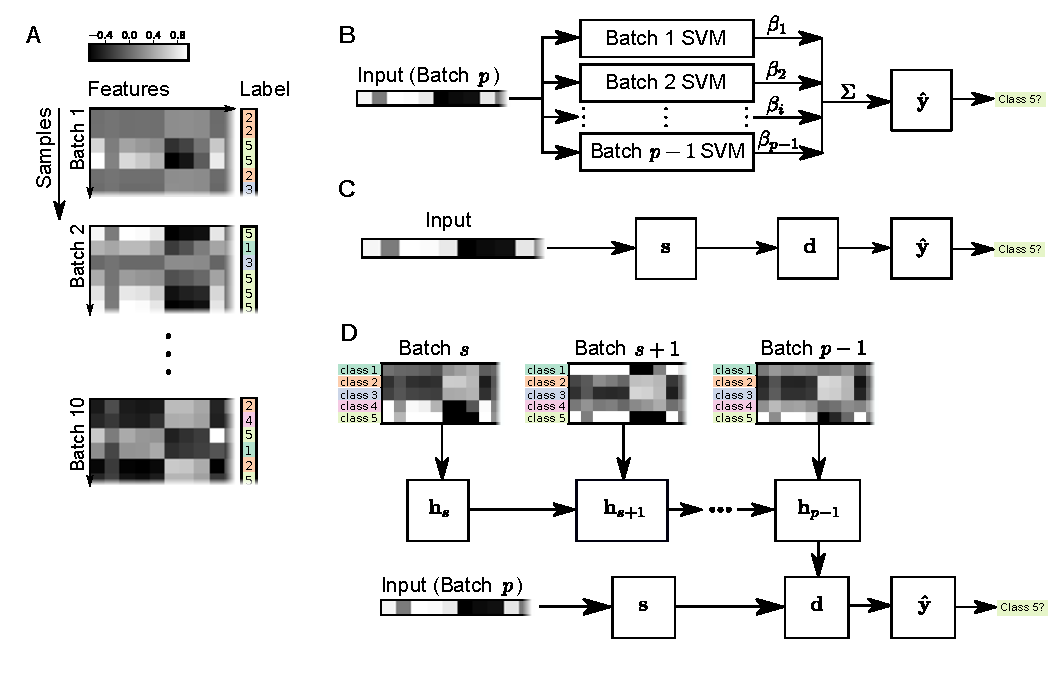
\includegraphics{fig_2.pdf}}
	\caption{\textbf{Neural network architectures.} (\textbf{A}.) Feature vectors and target labels were sampled from batches 1, 2, and 10 to illustrate the data format. Each sample is represented by a row of feature values from the sensor array in grayscale, along with the identifier (1 through 5) of the corresponding odor shown in color. The data consisted ten ordered batches, or data collection windows. (\textbf{B}.) A feature vector is input to a collection of SVMs, and the weighted sum of their class predictions is taken to be the output of the ensemble. (\textbf{C}.) A schematic of the feedforward model delineates feedforward progression of input through two hidden layers $\mathbf{s}$ and $\mathbf{d}$ followed by the output layer $\hat{\mathbf{y}}$. (\textbf{D}.) A schematic of the context model introduces a sequential processing of prior samples as a separate processing pathway. For each context batch from $s$ through $p-1$, one sample per odor class is chosen as a representative.}
\end{figure}

\subsection{Artificial neural networks}

While SVMs are standard machine learning, NNs have recently turned out more powerful, so the first step is to use them on this task instead of SVMs. In the classification task, the networks are evaluated by the similarity between the odor class label (1-5) and the network's output class label prediction given the unlabeled odor features. The output layer of the neural network is a five-dimensional vector of class scores, which represent the network's confidence attributed to each odor class label. The cross-entropy loss function combines the predicted class scores and the true odor label to form the network training signal. Assume that $\hat{\mathbf{y}}$ is the five-dimensional unnormalized class score vector, that $\hat{y}_i$ represents the score given to class $i$, and that $c$ is the identity of the true class label. Then the loss function is given
\begin{equation}
\mathcal{L} = - \hat{y}_c + \log \left( \sum_{i=1}^5 \exp(\hat{y}_i) \right).
\end{equation}

All neural networks in this section were trained using stochastic gradient descent with momentum \cite{rumelhart_learning_1986} on the loss function $\mathcal{L}$. The learning rate was set to $10^{-3}$ and the momentum factor to $0.9$. Networks were trained for 200 epochs under a weight decay factor of $10^{-2}$, which guards against overfitting the model to the training data \cite{pardo_remarks_2004}. The initial weights of each layer are sampled from a Gaussian distribution with zero mean and variance equal to the reciprocal of the number of units in the layer. The neural networks were implemented using the PyTorch backpropagation library \cite{paszke_pytorch_2019}.

Two neural network architectures are evaluated: a feedforward network as the baseline and the feedforward+context network that models the drift separately.

\subsubsection{The feedforward model}
The feedforward approach incorporates all available data into a single training set, disregarding the sequential structure between batches of the dataset. For each batch $T$, a feedforward network was trained using batches $1$ through $T-1$ as the training set and evaluated on batch $T$. 

The network is diagrammed in Figure 1C. It is input the 128-dimensional feature vector, $\mathbf{x}$, and calculates class scores, $\hat{\mathbf{y}}$, using two hidden layers: the 50-unit ``skill" layer, $\mathbf{s}$, and the 20-unit ``decision-making" layer, $\mathbf{d}$. Assume that $\mathbf{W}_{xs}$, $\mathbf{W}_{sd}$, and $\mathbf{W}_{dy}$ are matrices of dimensions $50\times 128$, $20\times 50$, and $20\times 5$, respectively, and that $\mathbf{b}_s, \mathbf{b}_d,$ and $\mathbf{b}_y$ are bias vectors of dimensions $50, 20,$ and $5$, respectively. Define $\relu$ to be the rectified linear activation function ($\relu(\mathbf{x})_i = \max(0, x_i)$). Then, the feedforward NN model is given by
\begin{equation}
\begin{split}
\mathbf{s}=\relu(\mathbf{W}_{xs}\cdot\mathbf{x}+\mathbf{b}_s), \\
\mathbf{d}=\relu(\mathbf{W}_{sd}\cdot\mathbf{s}+\mathbf{b}_d), \\
\hat{\mathbf{y}}=\mathbf{W}_{dy}\cdot\mathbf{d}+\mathbf{b}_y.
\end{split}
\end{equation}

This paper also presents the feedforward NN ensemble created in the same way as with SVMs. In the NN ensemble, $T-1$ feedforward networks are trained using one batch each for training. Each model is assigned a weight $\beta_i$ equal to its accuracy on batch $T-1$. The weighted sum of the model class scores is the ensemble class prediction. The model is then tasked to classify samples from batch $T$.


\subsubsection{The context model}
The feedforward+context NN model builds on the feedforward NN model by adding a recurrent processing pathway (Fig. 2D). Before classifying an unlabeled sample, the recurrent pathway processes a sequence of labeled samples from the preceding batches to generate a context representation, which is fed into the final feedforward processing layer. The recurrent layers are modified via backpropagation through time, and, in this manner, the recurrent pathway learns to generate representations that support classification.

The recurrent pathway is based on a recurrent neural network (RNN) approach. It reuses weights and biases across the steps of a sequence and can thus process variable-length sequences. The alternative was to use a long-short term memory (LSTM), which employs gating variables to better remember information in long sequences \cite{hochreiter_long_1997}. However, in preliminary experiments LSTM did not improve generalization accuracy significantly ($p\geq 0.05$, one-sided t-test blocked by batch), presumably because the sequences were relatively short (nine steps or less). The simple RNN was therefore used in the experiments presented in the paper. 

During training, for each unlabeled sample in the training set, a context sequence is sampled from the preceding batches. Assume the unlabeled training sample belongs to batch $p$, and $p \in \{ 2, 3, \ldots, T-1 \}$. Then, the final batch of the context sequence is $p-1$, and the start batch, $s$, is sampled uniformly among values $1, 2, \ldots, p-1$. At test time on batch $T$, all batches $1$ through $T-1$ are included for context; i.e., $s=1$, and $p=T-1$. Denote $\mathbf{x}_\mathrm{c}^{t,z}$ to be the feature vector sampled from batch $t$ of odor class $z$. The concatenation over all five classes in order forms a single vector for batch $t$ denoted $\mathbf{x}_\mathrm{c}^{t,:}$, which is the input to the RNN. The RNN iterates from batch $s$ to batch $p-1$ to form the hidden state by the recursive formula
\begin{equation}
\begin{split}
\mathbf{h}_s = \tanh(\mathbf{W}_{xh} \cdot \mathbf{x}_\mathrm{c}^{s,:} + \mathbf{b}_h),\\
\mathbf{h}_t = \tanh(\mathbf{W}_{hh}\cdot \mathbf{h}_{t-1} + \mathbf{W}_{xh} \cdot \mathbf{x}_\mathrm{c}^{t,:} +  \mathbf{b}_h).
\end{split}
\end{equation}

The output, $\mathbf{h}_{p-1}$,  of the recurrent pathway is integrated with the feedforward pathway. First, the unlabeled target sample $\mathbf{x}$ is processed in a 50-unit ``skill" layer, $\mathbf{s}$. Then, the 50-dimensional representation of $\mathbf{x}$ and the 10-dimensional context vector are combined in a 20-unit ``decision-making" layer, $\mathbf{d}$.  The class scores $\hat{\mathbf{y}}$ are a linear readout of $\mathbf{d}$. The entire model is thus given as
\begin{equation}
\begin{split}
\mathbf{s}=\relu(\mathbf{W}_{xs}\cdot\mathbf{x}+\mathbf{b}_{s}), \\
\mathbf{d}=\relu(\mathbf{W}_{sd}\cdot\mathbf{s} + \mathbf{W}_{hd}\cdot\mathbf{h}_{p-1}+\mathbf{b}_{d} ), \\
\hat{\mathbf{y}}=\mathbf{W}_{dy}\cdot\mathbf{d}+\mathbf{b}_{y}.
\end{split}
\end{equation}

The context processing pathway utilizes the sequential structure of the dataset via recurrent processing. This pathway is incorporated with a feedforward component to define the feedforward+context model as described above.

\begin{table*}[t]
\setlength{\tabcolsep}{1em}\begin{tabular}{lrrrrrrrrr}
& \multicolumn{6}{l}{Batch }\\
\cline{2-10}
 Model        &       3 &       4 &       5 &       6 &       7 &       8 &       9 &      10 &   $\mu$\\
\hline
 Feedforward   & 0.881          & 0.875          & 0.974          & \textbf{0.959} & 0.792          & 0.839          & 0.896          & 0.737          & 0.869          \\
 Feedforward+Context      & 0.882          & 0.869          & 0.975          & 0.947          & 0.820          & 0.864          & \textbf{0.939} & \textbf{0.763} & \textbf{0.882} \\
 Feedforward NN Ensemble  & \textbf{0.921} & \textbf{0.904} & 0.979 & 0.903          & 0.777          & 0.679          & 0.864          & 0.693          & 0.840          \\
 SVM Ensemble & 0.698          & 0.777          & 0.631          & 0.900          & 0.823 & \textbf{0.934} & 0.794          & 0.551          & 0.764          \\

\hline
\end{tabular}
\caption{\textbf{Mean generalization performance.} Listed is the classification accuracy (correct / total) of various models evaluated on the unseen testing data, i.e., batch $T$. The values represent the average accuracy over 30 trials. The final column lists the mean of the values for batches 3 through 10. A bolded value is significantly greater than the others in the same column ($p < 0.05$, two-sided pairwise t-test with correction for unequal variances).}
\end{table*}

\begin{figure}
	\frame{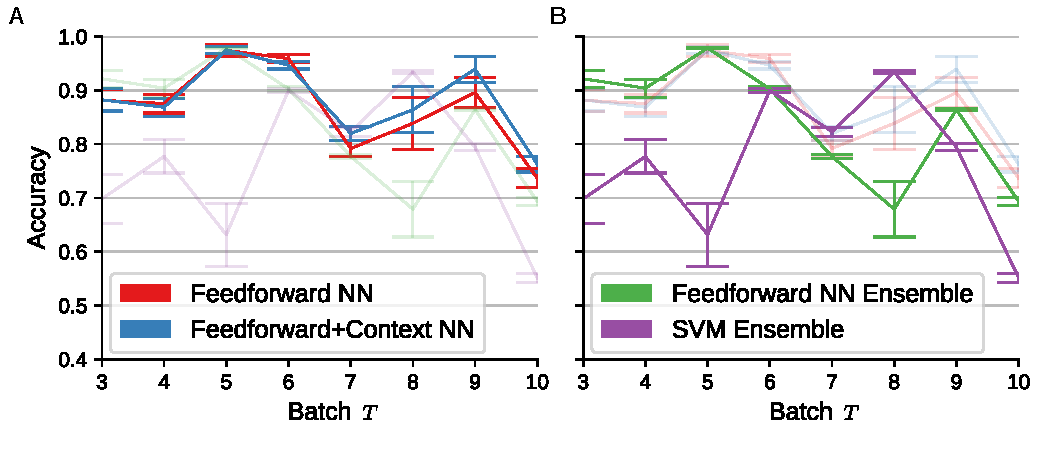
\includegraphics{fig_3.pdf}}
	\caption{\textbf{Generalization accuracy.} The generalization accuracy of each model was evaluated on batch $T$. For each model type and every batch, 30 models were trained. The line represents the average over the 30 trials, and the error bar is the 95\% confidence interval. (\textbf{A}.) The feedforward and feedforward+context models are shown with the other models faded out. The context most contributes to performance in the later batches, which offer the longest context sequences. (\textbf{B}.) The SVM ensemble and feedforward NN ensemble models are shown with the results from (A) are shown faded out. Both ensemble models are variable in performance between batches. }
\end{figure}

\section{Experiments}
A series of experiments were carried out to evaluate the following hypotheses:
\begin{enumerate}
\item Sensor drift has a sequential structure.
\item Neural network ensembles offer better generalization properties than do SVM ensembles.
\item The inclusion of context improves the generalization performance of neural networks.
\end{enumerate}

\subsection{Drift demonstration}
First, the effect of sensor drift on classification accuracy is demonstrated using classifiers trained on a single batch. For each batch $1$ through $10$, a feedforward model was trained on that batch. Training of a new model was repeated 30 times on each batch. The accuracy of all classifiers were evaluated on every batch. Networks trained on batches 2, 4, 6, and 8 were plotted (Fig. 1B).  The accuracy data was reformulated as a function of the distance between the train batch and the test batch (Fig. 1C). As expected, the accuracy decreases with the time gap between training and testing, demonstrating that, indeed, sensor drift progresses over time.

\subsection{Ensemble models}

The second comparison is between the weighted ensembles of SVMs, i.e., the state of the art \cite{vergara_chemical_2012}, and the weighted ensembles of neural networks. For each batch, an SVM and a feedforward neural network were trained with that batch as the training set. Weighted ensembles were constructed for each batch $T$ by assigning weights to the models trained on batches 1 through $T-1$. Training of a new ensemble and evaluation were repeated for thirty trials. The generalization accuracy classifying samples in batch $T$ was reported for the neural network ensemble (Fig. 3B, Table 1, \textit{Feedforward NN Ensemble}) and for the SVM ensemble (Fig. 3B, Table 1, \textit{SVM Ensemble}). The neural network ensemble model had a significantly greater mean generalization accuracy than the SVM ensemble model ($p < 0.05$, two-sided t-test blocked by batch), and the neural network ensemble model achieved the highest generalization accuracy among all models on batches 3 and 4 ($p < 0.05$, pairwise two-sided t-test). The results indicate that while NN ensembles outperform SVM ensembles on average, there is significant batch to batch variability.

\subsection{Context}
For each batch $T$ from 3 through 10, the batches $1, 2, \ldots, T-1$ were used to train feedforward NN and feedforward+context NN models for 30 trials. The accuracy was measured classifying examples from batch $T$ (Fig. 3A, Table 1, \textit{Feedforward NN} and \textit{Feedforward+Context NN}). The context models achieved a greater average accuracy, computed as the mean over all batches tested of the average accuracy in that batch ($p<0.05$, two-sided t-test blocked by batch). In batch 6, the feedforward NN outperformed the feedforward+context NN, while the feedforward+context NN achieved greater performance in batches 7, 9, and 10 (two-sided t-tests, $p<0.05$).

\section{Discussion}
The purpose of this study was to demonstrate that context can improve generalization in neural networks. In a setting with sequential sensor drift, several gas classifier models were evaluated on future data. This task reflects the practical goal to deploy an artificial nose in a dynamic environment without recalibration.

Extending the previous SVM ensemble model \cite{vergara_chemical_2012}, a similar ensemble was formed from modern deep learning networks. The accuracy improvements suggested that neural networks are indeed more accurate than SVMs in this task.

The main comparison, however, was between the feedforward NN and feedforward+context NN models. The context-based network extracts features from preceding batches in sequence in order to model how the sensors drift over time. When added to the feedforward NN representation, such contextual information resulted in improved generalization accuracy. This benefit was larger in later batches where the drift was the largest and where there was a longer context to use as a basis for generalization.

While context did introduce more parameters to the model ($7{,}575$ parameters without context versus $14{,}315$ including context), the models is comparatively small next to million-parameter modern deep learning networks and is trainable in a number of hours on a CPU. When units were added to the ``skill" layer of the feedforward NN model until the total number of parameters reached $14{,}429$, the larger model was not significantly better ($p\geq 0.05$, one-sided t-test blocked by batch). This reinforces the idea that the benefit may be attributed to context, and not to the size of the network.

The estimation of context by learned temporal patterns should be most effective when the environment results in recurring or cyclical patterns, such as in cyclical variations of temperature and humidity and regular patterns of human behavior generating interferents. In such cases, the recurrent pathway can identify useful patterns analagously to how cortical regions help the olfactory bulb filter out previously seen background information \cite{adams_top-down_2019}. A context-based approach will be applied to longer-timescale data and to environments with cyclical patterns. 

The current design of the context-based network relies on labeled data because the odor samples for a given class are presented as ordered input to the context layer. However, the model can be modified to be trained on unlabeled data, simply by allowing arbitrary data samples as input to the context layer. This design introduces variation in training inputs, which makes it harder to learn consistent context patterns. For this task, semi-supervised learning techniques, such as self-labeled samples, may help. If the context layer can process unlabeled data, then it is no longer necessary to include every class in every batch. The full 6-gas sensor drift dataset can be used, as well as other unbalanced and therefore realistic datasets.

\section{Conclusion}
Sensor drift poses a problem for gas sensing systems, which, to stay reliable over time while incurring low maintenance costs, may benefit from pattern detection algorithms that generalize well to new settings. This paper introduced a recurrent neural network architecture which processes a sequence of previously seen gas recordings to generate information about the current context. The information improved performance on a classification task when generalizing to an unseen setting modified by sensor drift. Reducing the impact of sensor drift on classification accuracy, context models may extend the effective lifetime of gas identification systems and similar systems in other domains.

\section{Acknowledgments}
This research was made possible by assistance from the Defense Advanced Research Projects Agency (DARPA) Lifelong Learning Machines program under grant HR0011-18-2-0024.

%\bibliographystyle{unsrt}
\bibliographystyle{myplain}

\begin{thebibliography}{10}

\bibitem{adams_top-down_2019}
W. Adams, J.~N. Graham, X. Han, and H. Riecke.
\newblock Top-down inputs drive neuronal network rewiring and context-enhanced
  sensory processing in olfaction.
\newblock {\em PLOS Computational Biology}, 15(1):e1006611, January 2019.

\bibitem{barsan_metal_2007}
N. Barsan, D. Koziej, and U. Weimar.
\newblock Metal oxide-based gas sensor research: {How} to?
\newblock {\em Sensors and Actuators B: Chemical}, 121(1):18--35, January 2007.

\bibitem{chang_libsvm_2011}
C.-C. Chang and C.-J. Lin.
\newblock {LIBSVM}: {A} library for support vector machines.
\newblock {\em ACM Transactions on Intelligent Systems and Technology},
  2(3):1--27, April 2011.

\bibitem{dickinson_current_1998}
T.~A. Dickinson, J. White, J.~S. Kauer, and D.~R. Walt.
\newblock Current trends in `artificial-nose' technology.
\newblock {\em Trends in Biotechnology}, 16(6):250--258, June 1998.

\bibitem{fu_pattern_2007}
J. Fu, G. Li, Y. Qin, and W.~J. Freeman.
\newblock A pattern recognition method for electronic noses based on an
  olfactory neural network.
\newblock {\em Sensors and Actuators B: Chemical}, 125(2):489--497, August
  2007.

\bibitem{hochreiter_long_1997}
S. Hochreiter and J. Schmidhuber.
\newblock Long short-term memory.
\newblock {\em Neural Computation}, 9(8):1735--1780, November 1997.

\bibitem{imam_rapid_2019}
N. Imam and T.~A. Cleland.
\newblock Rapid online learning and robust recall in a neuromorphic olfactory
  circuit.
\newblock {\em arXiv:1906.07067 [cs, q-bio]}, June 2019.
\newblock arXiv: 1906.07067.

\bibitem{kay_odor-_1999}
L.~M. Kay and G. Laurent.
\newblock Odor- and context-dependent modulation of mitral cell activity in
  behaving rats.
\newblock {\em Nature Neuroscience}, 2(11):1003--1009, November 1999.

\bibitem{marco_recent_2009}
S. Marco and A. Gutierrez‐Gálvez.
\newblock Recent {Developments} in the {Application} of {Biologically}
  {Inspired} {Computation} to {Chemical} {Sensing}.
\newblock {\em AIP Conference Proceedings}, 1137(1):151--154, May 2009.

\bibitem{marco_signal_2012}
S. Marco and A. Gutierrez-Galvez.
\newblock Signal and {Data} {Processing} for {Machine} {Olfaction} and
  {Chemical} {Sensing}: {A} {Review}.
\newblock {\em IEEE Sensors Journal}, 12(11):3189--3214, November 2012.

\bibitem{pardo_remarks_2004}
M. Pardo and G. Sberveglieri.
\newblock Remarks on the use of multilayer perceptrons for the analysis of
  chemical sensor array data.
\newblock {\em IEEE Sensors Journal}, 4(3):355--363, June 2004.

\bibitem{paszke_pytorch_2019}
A. Paszke, S. Gross, F. Massa, A. Lerer, J. Bradbury, G. Chanan, T. Killeen, Z.
  Lin, N. Gimelshein, L. Antiga, A. Desmaison, A. Kopf, E. Yang, Z. DeVito, M.
  Raison, A. Tejani, S. Chilamkurthy, B. Steiner, L. Fang, J. Bai, and S.
  Chintala.
\newblock {PyTorch}: {An} imperative style, high-performance deep learning
  library.
\newblock In H. Wallach, H. Larochelle, A. Beygelzimer, F. Alché-Buc, E. Fox,
  and R. Garnett, editors, {\em Advances in {Neural} {Information} {Processing}
  {Systems} 32}, pages 8026--8037. Curran Associates, Inc., 2019.

\bibitem{pedregosa_scikit-learn_2011}
F. Pedregosa, G. Varoquaux, A. Gramfort, V. Michel, B. Thirion, O. Grisel, M.
  Blondel, P. Prettenhofer, R. Weiss, V. Dubourg, J. Vanderplas, A. Passos, D.
  Cournapeau, M. Brucher, M. Perrot, and E. Duchesnay.
\newblock Scikit-learn: {Machine} {Learning} in {Python}.
\newblock {\em Journal of Machine Learning Research}, 12(Oct):2825--2830, 2011.

\bibitem{rumelhart_learning_1986}
D.~E. Rumelhart, G.~E. Hinton, and R.~J. Williams.
\newblock Learning representations by back-propagating errors.
\newblock {\em Nature}, 323(6088):533--536, October 1986.

\bibitem{shipley_functional_1996}
M.~T. Shipley and M. Ennis.
\newblock Functional organization of olfactory system.
\newblock {\em Journal of Neurobiology}, 30(1):123--176, 1996.

\bibitem{thomas-danguin_perception_2014}
T. Thomas-Danguin, C. Sinding, S. Romagny, F. El~Mountassir, B. Atanasova, E.
  Le~Berre, A.-M. Le~Bon, and G. Coureaud.
\newblock The perception of odor objects in everyday life: a review on the
  processing of odor mixtures.
\newblock {\em Frontiers in Psychology}, 5, June 2014.

\bibitem{vergara_chemical_2012}
A. Vergara, S. Vembu, T. Ayhan, M.~A. Ryan, M.~L. Homer, and R. Huerta.
\newblock Chemical gas sensor drift compensation using classifier ensembles.
\newblock {\em Sensors and Actuators B: Chemical}, 166-167:320--329, May 2012.

\bibitem{vito_pattern_2016}
S.~D. Vito, M. Falasconi, and M. Pardo.
\newblock Pattern {Recognition}.
\newblock In {\em Essentials of {Machine} {Olfaction} and {Taste}}, pages
  175--217. John Wiley \& Sons, Ltd, 2016.

\end{thebibliography}

%\renewcommand\bibname{Reference}
\end{document}